\documentclass[tikz,border=8pt]{standalone}
% Shared look for every TikZ diagram. Load with \input{../../tools/tikz-style.tex}
\usepackage[sfdefault]{roboto}
\usetikzlibrary{arrows.meta, positioning, shapes.geometric, calc, fit, backgrounds}
\definecolor{cblue}{HTML}{4C78A8}
\definecolor{corange}{HTML}{F58518}
\definecolor{cgreen}{HTML}{54A24B}
\definecolor{cred}{HTML}{E45756}
\definecolor{cpurple}{HTML}{B279A2}
\definecolor{cgrey}{HTML}{6B6B6B}
\tikzset{
  every picture/.style={font=\sffamily, line width=1.2pt},
  box/.style={draw=#1, fill=#1!12, rounded corners=4pt, align=center, inner sep=7pt, minimum height=1.1cm},
  box/.default=cgrey,
  arrow/.style={-{Stealth[length=3mm]}, draw=cgrey, line width=1.4pt},
  title/.style={font=\sffamily\bfseries\Large},
  note/.style={font=\sffamily\small, text=cgrey, align=center},
}
\AtBeginDocument{\hyphenpenalty=10000 \exhyphenpenalty=10000}

% The idea of pure pursuit at the start of the course: the car's rear axle at (0, 1), heading along x, the course
% along y = 0. A circle of radius ld = 4 m around the rear axle meets the course ahead at (3.873, 0): the
% look-ahead point. The nearest course point is (0, 0), 1.0 m to the right. 1 unit = 1 m.
\begin{document}
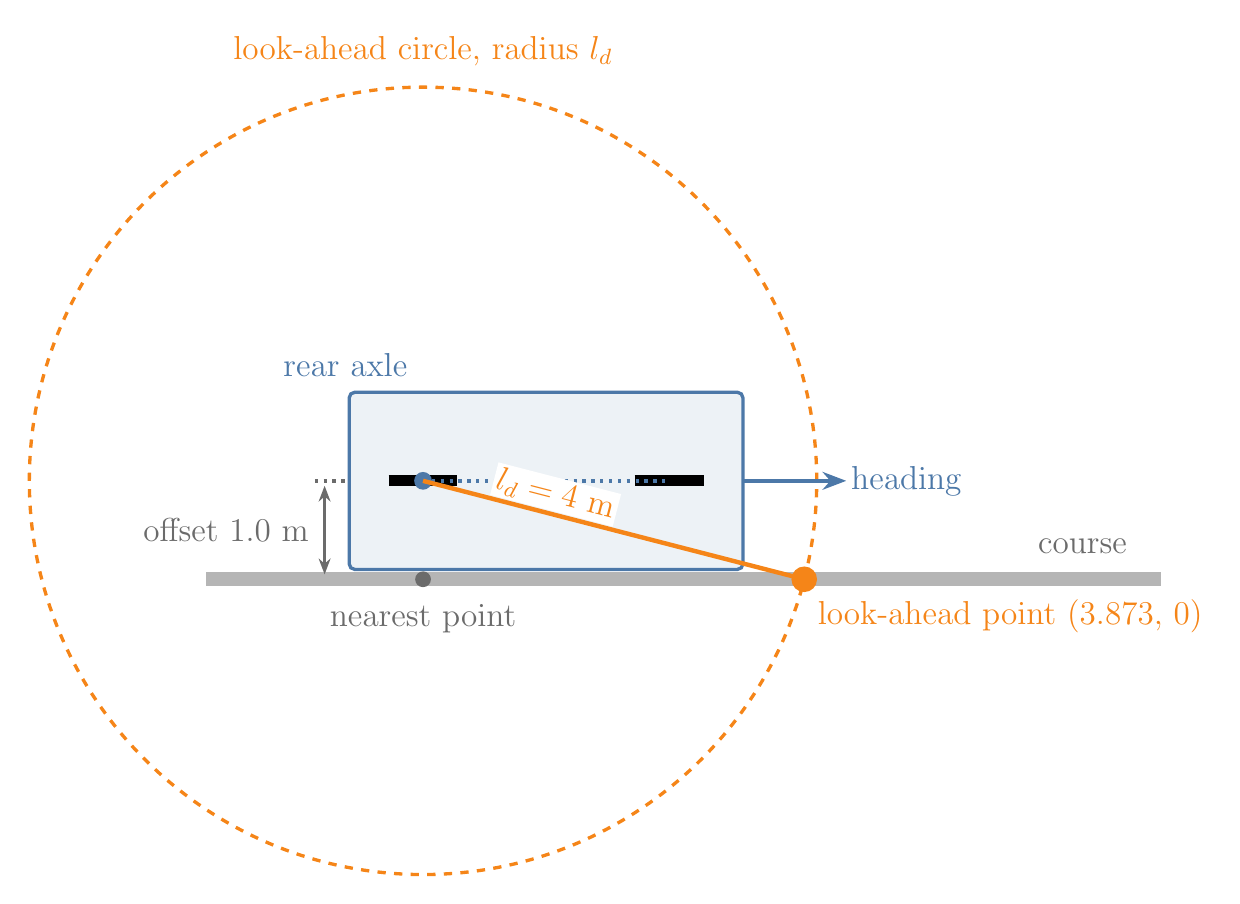
\begin{tikzpicture}[scale=1.25, every node/.append style={font=\large}]
  % course
  \draw[cgrey!50, line width=5pt] (-2.2,0) -- (7.5,0);
  \node[cgrey, anchor=south] at (6.7,0.15) {course};
  % look-ahead circle
  \draw[corange, dashed, line width=1.2pt] (0,1) circle (4);
  % car body: 4.0 m long, 1.8 m wide, rear axle 0.75 m from the back
  \draw[cblue, fill=cblue!10, rounded corners=2pt] (-0.75,0.1) rectangle (3.25,1.9);
  \draw[black, line width=4pt] (-0.35,1) -- (0.35,1);
  \draw[black, line width=4pt] (2.15,1) -- (2.85,1);
  \draw[cblue, dotted] (0,1) -- (2.5,1);
  \fill[cblue] (0,1) circle (0.09);
  \node[cblue, anchor=south east] at (-0.05,1.95) {rear axle};
  % heading arrow
  \draw[-{Stealth[length=3mm]}, cblue, line width=1.6pt] (3.25,1) -- (4.3,1) node[right, fill=white, inner sep=1pt] {heading};
  % nearest point and offset
  \fill[cgrey] (0,0) circle (0.08);
  \draw[cgrey, line width=1pt, {Stealth[length=2mm]}-{Stealth[length=2mm]}] (-1.0,0.05) -- (-1.0,0.95); \draw[cgrey, dotted] (-1.1,1) -- (-0.75,1);
  \node[cgrey, anchor=east] at (-1.05,0.5) {offset 1.0 m};
  \node[cgrey, anchor=north] at (0,-0.15) {nearest point};
  % look-ahead distance and point
  \draw[corange, line width=1.6pt] (0,1) -- (3.873,0);
  \node[corange, anchor=south, rotate=-14.5, fill=white, inner sep=1pt] at (1.3,0.68) {$l_d = 4$ m};
  \fill[corange] (3.873,0) circle (0.13);
  \node[corange, anchor=north west] at (3.9,-0.1) {look-ahead point (3.873, 0)};
  \node[corange, anchor=south] at (0,5.1) {look-ahead circle, radius $l_d$};
\end{tikzpicture}
\end{document}
